\chapter{Experiments and Results}
\label{chapter:experiments}

So far we have discussed the CCD approach in detail. In this chapter,
the experimental evaluation of the CCD algorithm and the naive CCD tracker will be provided. In previous
chapter, we have introduced the application of the CCD algorithm and
its variant. Experiments have been performed on the PR2. we apply the
CCD approach to three different kinds of model fitting and tracking
problems:

\begin{enumerate}
\item Contour convergence on still image
\item Tracking initialization from sift features
\item Tracking initialization from 3D point cloud
\end{enumerate}

We analyze the performance of the approach in terms of robustness,
accuracy and runtime. This is followed the comparison between the CCD
approach and  other state-of-the-art methods.
% by the experimental evaluation of the CCD
% algorithm. presents the evaluation of the naive CCD
% tracker and 

\section{Contour convergence on still image}
\label{sec:ES}

As mentioned in related work, the CCD algorithm is an effective
segmentation method like other model-based segmentation algorithms.

A segmentation of an image $I: \Omega \subset R^2 \longrightarrow R$
is the partitioning of its domain into homogeneous regions
$\Omega_1,\ldots, \Omega_n \subset \Omega$. There are many pratical
applications of image segmentation, such as medical imaging, object
tracking, face recognition, fingerprint recognition, machine vison and
so on. In this thesis, we concern its application in object tracking.
In many cases segmentation is the bottleneck when trying to tracking a
object. Many segmentation methods are developed, however, there is not
general solution to the segmentation problem. In the real world,
segmentation problems will often require much domain knowledge before
a successful segmentation can be performed. The CCD algorithm is just
such a method which is combined with the prior knowledge. By
converting a pure segmentation problem to a problem in pattern
recognition, a large amount of techniques in the field of pattern
recognition are introduced to solve segmentation problems, which are
proved to be effective and helpful. Compared with other segmentation
methods, such as intensive-based method,  cluster method, region-based
method and compression-based methods, the CCD algorithm has following
advantages:
\begin{itemize}
\item restrict segmentation problem to a limited explicit region, it is helpful
  to decrease the computation cost.
\item probabilistic representation of the variation of the registered
  samples could be easily given, thus statistical inference between
  the model and the image will be applied. All these are helpful to
  improve the segmentation results.
\item The CCD algorithm achieves sub-pixel accuracy and high
  robustness because only a relatively small fraction of the pixels is
  taken into account in the end of iteration.
\end{itemize}

In the following, we apply the proposed CCD algorithm to 4 kind of
objects:
\begin{enumerate}
\item segmentation of a ball
\item segmentation of 3-D object
\item segmentation of a transparent object
\item fitting a deformable models
\end{enumerate}

\subsection{Segmenation of a ball}
\label{sec:sb}
Like other model-based method, we model a contour of the ball as the
prior knowledge. Due to existing general contour for spherical object,
besides manual initialization, we can use some built-in function in
OpenCV library to generate the contour with given center and
radius. According the definition of prior distribution, it is required
to guarantee that the hypothesis is in the range of the variation of
registered sample, namely, the initial contour can not be too far away
from the target.

\begin{figure} 
  \begin{minipage}[t]{0.45\linewidth} 
    \centering 
        \subfloat[iteration 1]{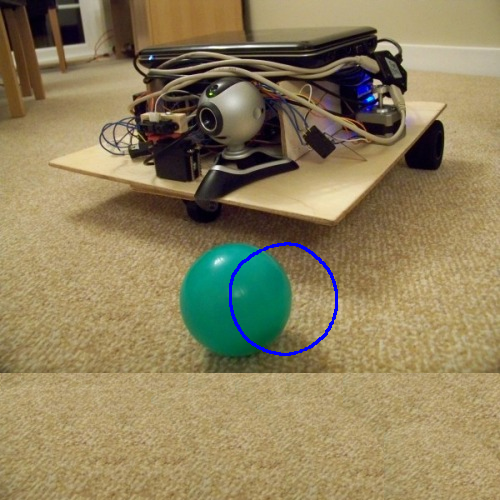
\includegraphics[width=2.0in]{images/ball/0.png}}
  \end{minipage}% 
  \begin{minipage}[t]{0.45\linewidth} 
    \centering 
    \subfloat[iteration 3]{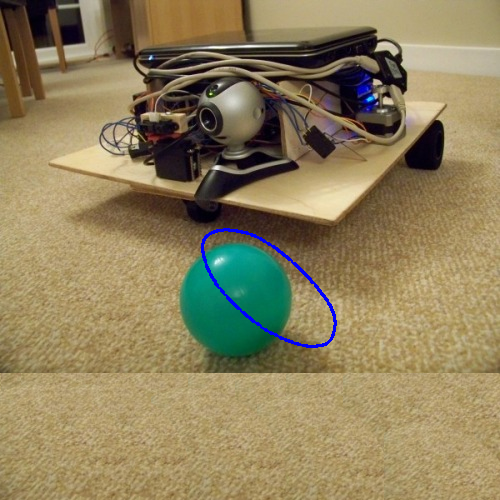
\includegraphics[width=2.0in]{images/ball/2.png}}
  \end{minipage} 
  \begin{minipage}[t]{0.45\linewidth} 
    \centering 
    \subfloat[iteration 7]{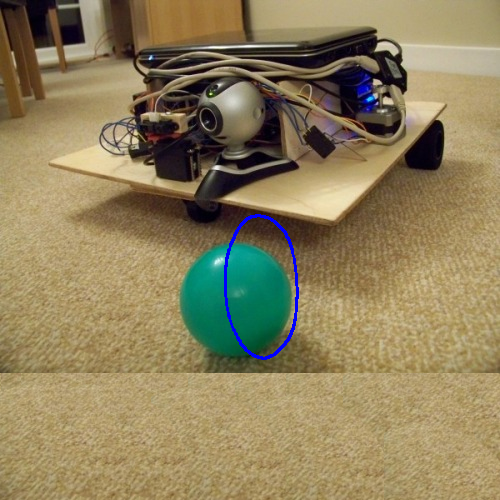
\includegraphics[width=2.0in]{images/ball/6.png}}
  \end{minipage} 
  \begin{minipage}[t]{0.45\linewidth} 
    \centering 
    \subfloat[iteration 16]{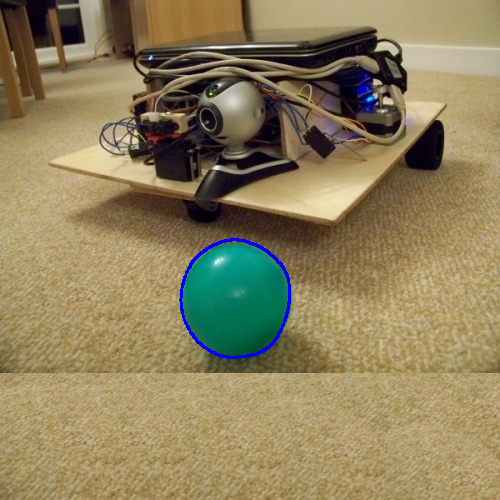
\includegraphics[width=2.0in]{images/ball/15.png}}
  \end{minipage} 
\caption{segmentation of a ball}
\end{figure}

In figure 6.1, we intentionally set a hypothesis which is far away
from the ball, but after about 15 iteration, we successfully fit the
contour the edge of the ball. For the sake of a ground truth we need
investigate the pixels used in the iterations. The figure 6.2 show
that only a small number of pixels is taken into account after the
contour starts to converge. However, these pixels contain the
necessary information for refining the fit. Because the pixels used
to compute became smaller and smaller, at last, it is supposed that
only a small number of pixels near the boundary are considered. The
CCD algorithm can achieve high sub-pixel accuracy.

\begin{figure} 
  \begin{minipage}[t]{0.45\linewidth} 
    \centering 
    \subfloat[iteration 1]{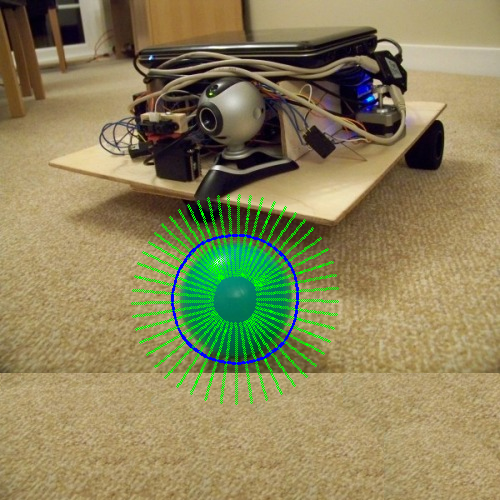
\includegraphics[width=2.0in]{images/ball_normal/0.png}}
  \end{minipage}% 
  \begin{minipage}[t]{0.45\linewidth} 
    \centering 
    \subfloat[iteration 3]{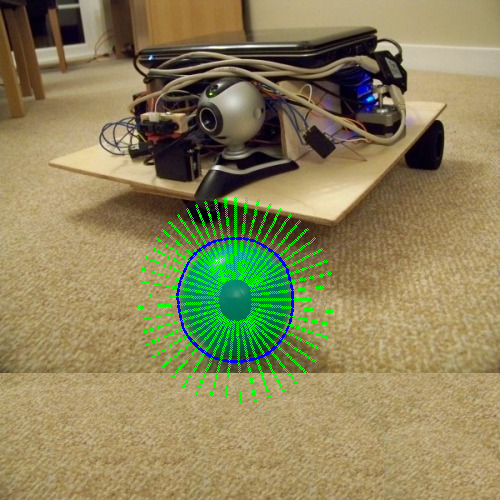
\includegraphics[width=2.0in]{images/ball_normal/1.png}}
  \end{minipage} 
  \begin{minipage}[t]{0.45\linewidth} 
    \centering 
    \subfloat[iteration 5]{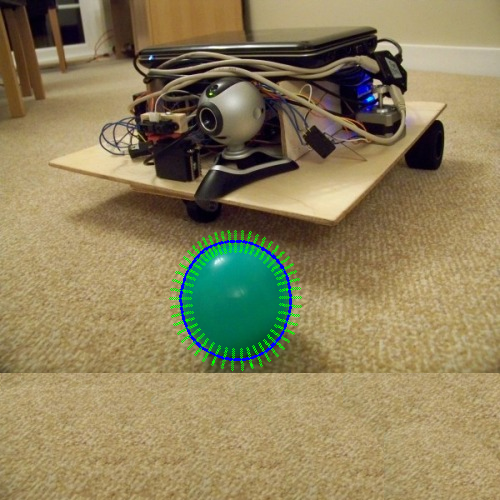
\includegraphics[width=2.0in]{images/ball_normal/3.png}}
  \end{minipage} 
  \begin{minipage}[t]{0.45\linewidth} 
    \centering 
    \subfloat[iteration 6]{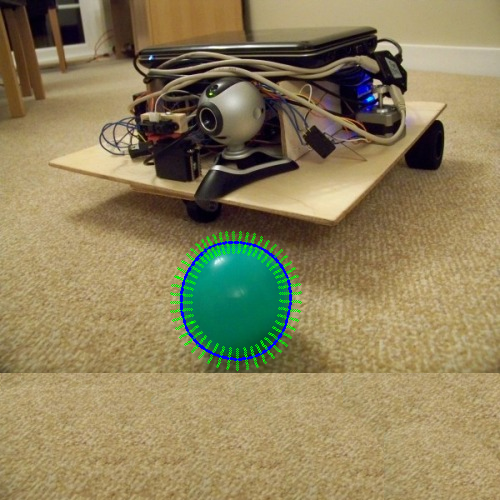
\includegraphics[width=2.0in]{images/ball_normal/4.png}}
  \end{minipage} 
\caption{pixels used in each iteration}
\end{figure}



\subsection{Segmenation of a 3-D obejct}
\label{sec:s3o}
In the experiments of segmentation of a spherical object, a planar
affine space of contour is generated. It works very well because the
contour of the ball is always a circle, there is not parallax effect
for such objects. In this case, a 6-dimension model parameters vector
can cope with basic geometrical transformation of a object. However,
clearly it can not be expected to suffice for non-planar
surfaces. Imagine such a scenario, we generate the  planar affine
space contour of a non-planar cube in the fist view. In the
subsequent view the outline of the cube does not lie in the old
space. Due the parallax effect the a mismatch in the fitted contour
will be expected to detect. This can be evidenced in the by the
fitting experiments in figure 6.3.
\begin{figure}[htbp]
  \centering
    \centering 
    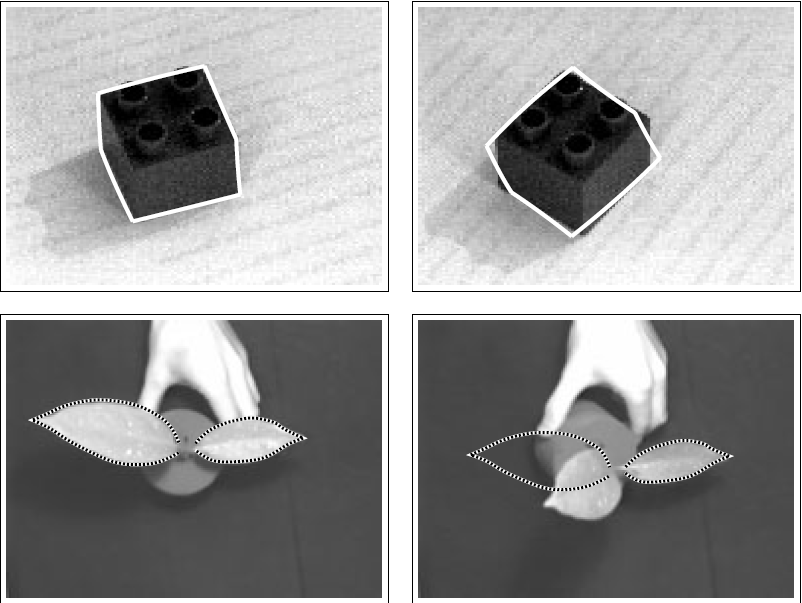
\includegraphics[width=\linewidth]{images/mismatch.png}
  \caption{Planar space can not encompassed a general non-planar contour}
\end{figure}


The new 3-dimensional affine shape-space with 8 degree of freedom,
made up of the 6-parameter planar affine space and a two-parameter
extension, is introduced to cope with such problem. Two added components
account for the depth variation that is not visible in the template
view. If tacking the two new parameters to the shape matrix, the form
of shape matrix for 3-dimensional case can be given by

\begin{equation}
  \label{eq:4.18}
  A =
  \begin{bmatrix}
    1 & 0 & P_0^x & 0 & 0 & P_0^y & P_0^z & 0\\
    0 & 1 & 0 & P_0^y & P_0^x & 0 & 0  & P_0^z
  \end{bmatrix}
\end{equation}

The three-dimensional affine shape-space model parameters have
the following interpretation

\begin{equation}
  \label{eq:4.19}
  \mathbf{\Phi} =  (T_1, T_2, M_{11} - 1, M_{22} - 1, M_{21}, M_{12}, \nu_1, \nu_2)
\end{equation}

The expanded space now encompasses the outlines of all views of the three-dimensional
outline, evidenced by figure 6.4

\begin{figure} 
  \begin{minipage}[t]{0.45\linewidth} 
    \centering 
    \subfloat[iteration 1]{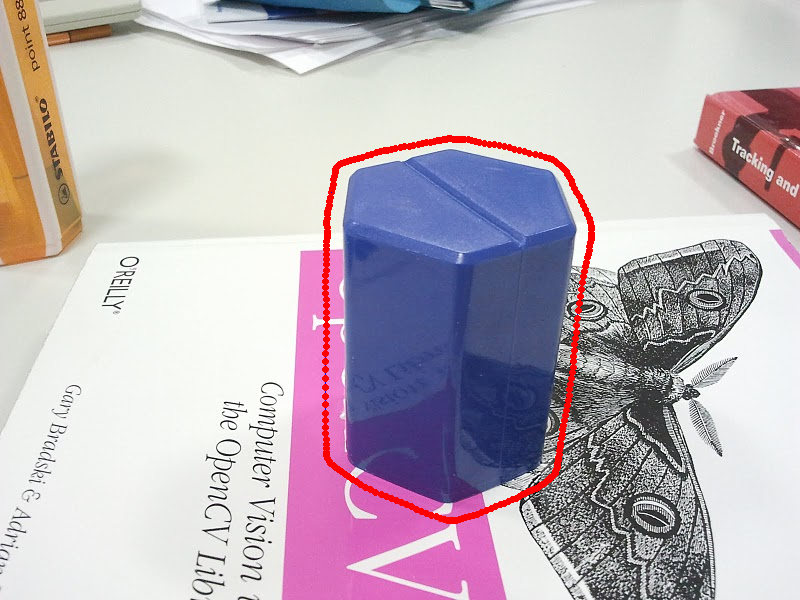
\includegraphics[width=2.0in]{images/container/0.png}}
  \end{minipage}% 
  \begin{minipage}[t]{0.45\linewidth} 
    \centering 
    \subfloat[iteration 2]{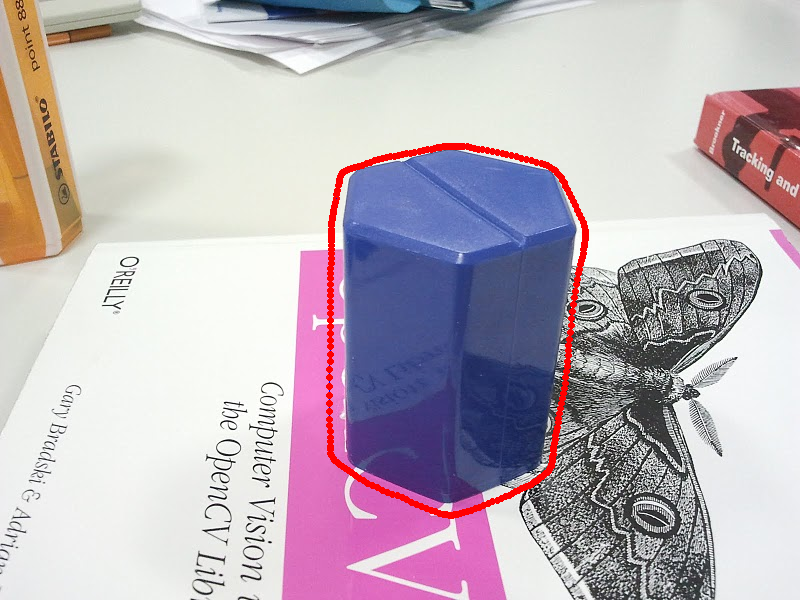
\includegraphics[width=2.0in]{images/container/1.png}}
  \end{minipage} 
  \begin{minipage}[t]{0.45\linewidth} 
    \centering 
    \subfloat[iteration 4]{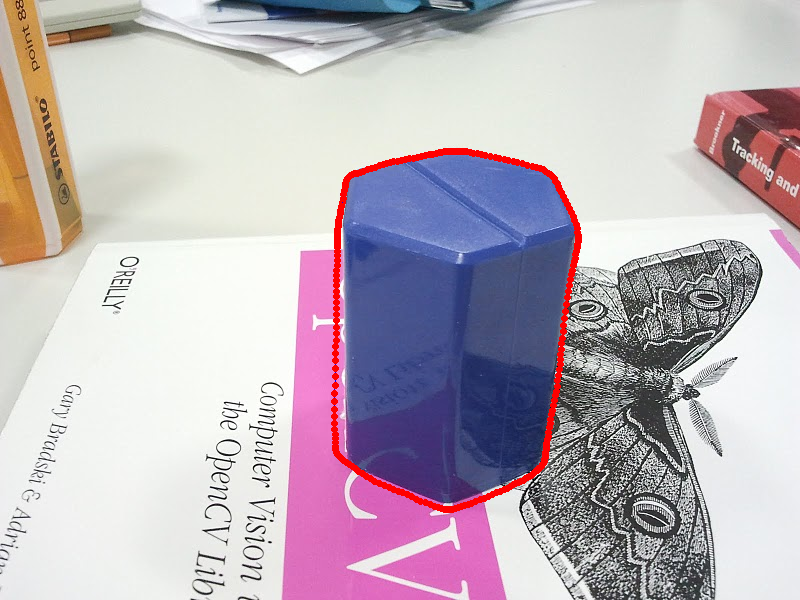
\includegraphics[width=2.0in]{images/container/2.png}}
  \end{minipage} 
  \begin{minipage}[t]{0.45\linewidth} 
    \centering 
    \subfloat[iteration 7]{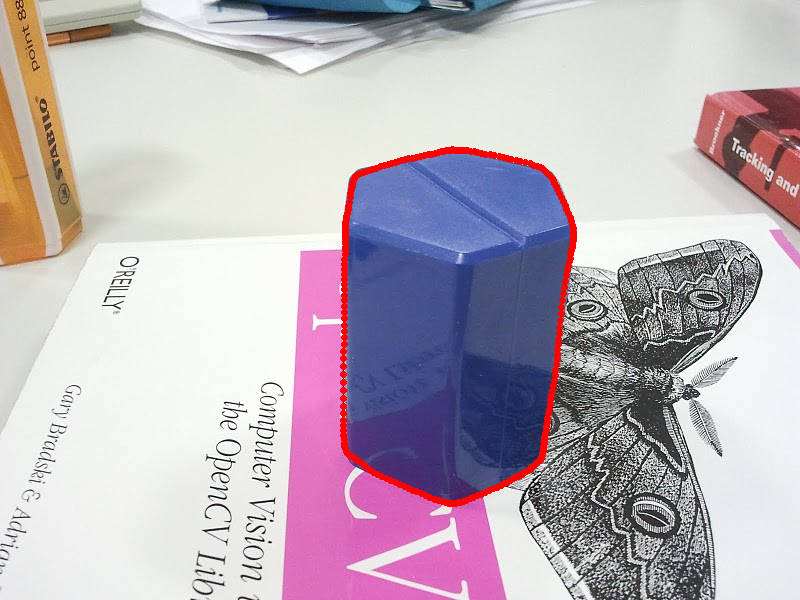
\includegraphics[width=2.0in]{images/container/5.png}}
  \end{minipage} 
\caption{segmentation of a non-planar object}
\end{figure}

\subsection{Segmenation of a transparent obejct}
\label{sec:sto}
In this thesis, local statistical information is collected in terms of
pixel intensity in the vicinity of a contour, therefore, the CCD
algorithm works not well for transparent. In this experiment, the
target is a cola bottle whose upper part is nearly transparent and the
lower part is opaque. The result in 6.5 shows that the CCD algorithm
can segment the lower part but can not encompass the contour in the
upper part completely. However, because the model only have 6 (or 8
for 3-dimensional object) degree of freedom, the convergence of other
part will effect the fitting in the transparent part such that we can
detect that the convergence happened in the transparent part.


\begin{figure} 
  \begin{minipage}[t]{0.45\linewidth} 
    \centering 
    \subfloat[iteration 1]{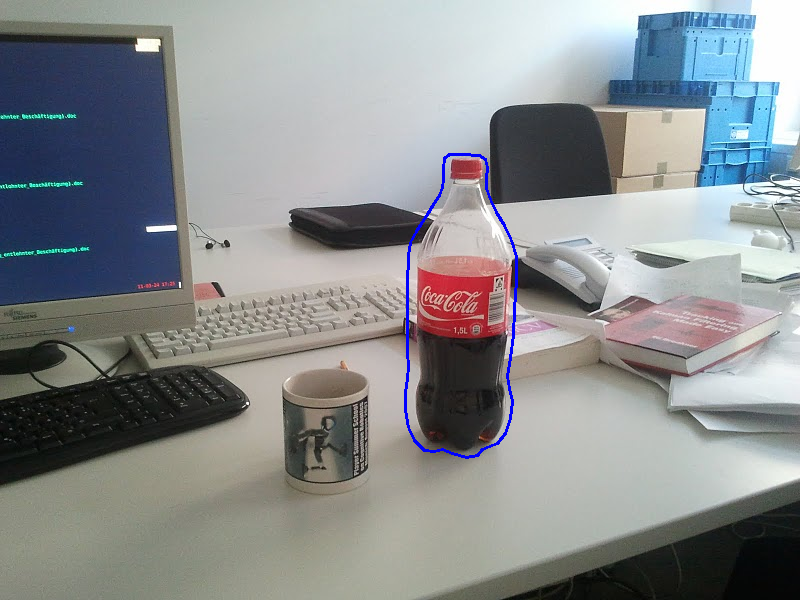
\includegraphics[width=2.0in]{images/bottle/0.png}}
  \end{minipage}% 
  \begin{minipage}[t]{0.45\linewidth} 
    \centering 
    \subfloat[iteration 2]{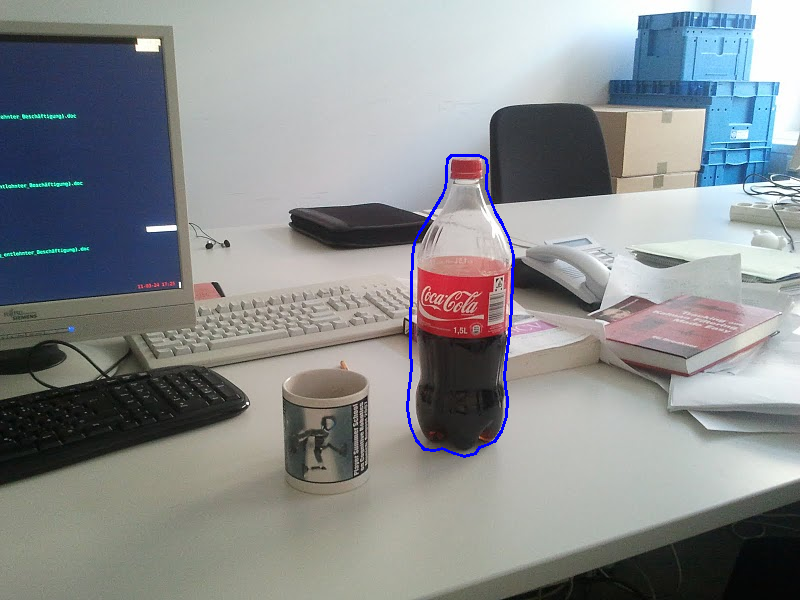
\includegraphics[width=2.0in]{images/bottle/1.png}}
  \end{minipage} 
  \begin{minipage}[t]{0.45\linewidth} 
    \centering 
    \subfloat[iteration 3]{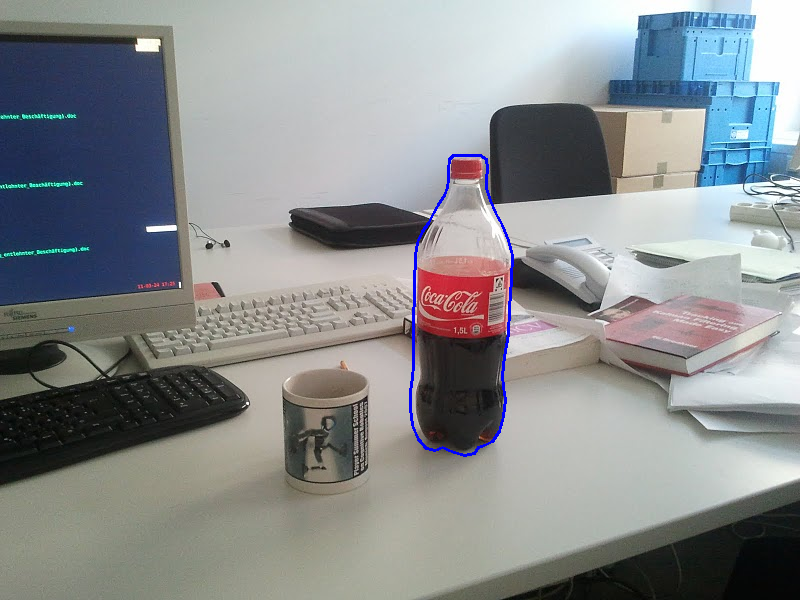
\includegraphics[width=2.0in]{images/bottle/2.png}}
  \end{minipage} 
  \begin{minipage}[t]{0.45\linewidth} 
    \centering 
    \subfloat[iteration 21]{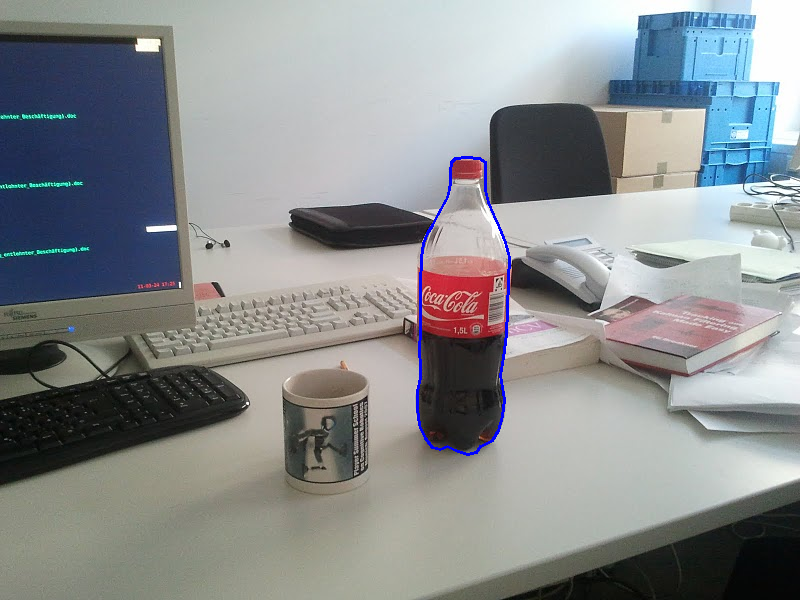
\includegraphics[width=2.0in]{images/bottle/20.png}}
  \end{minipage} 
\caption{segmentation of a transparent bottle}
\end{figure}


\subsection{Fitting a rigid wire frame}
\label{sec:fdo}

The next example shows that the CCD algorithm is not only able to exploit object contours,
but it can also use internal model edges separating multiple, possibly dependent, image regions.
We fit a rigid wire frame model to the image depicted in Figure 5.12a. The degrees of freedom
are the 8 pose parameters. The CCD algorithm reliably estimates the pose of the box despite
the partial occlusion. Again, a gradient-based edge detector (Steger, 2000) yields multiple false
positive and false negative errors, see Figure 6.6

\begin{figure} 
  \begin{minipage}[t]{0.45\linewidth} 
    \centering  
    \subfloat[iteration 1]{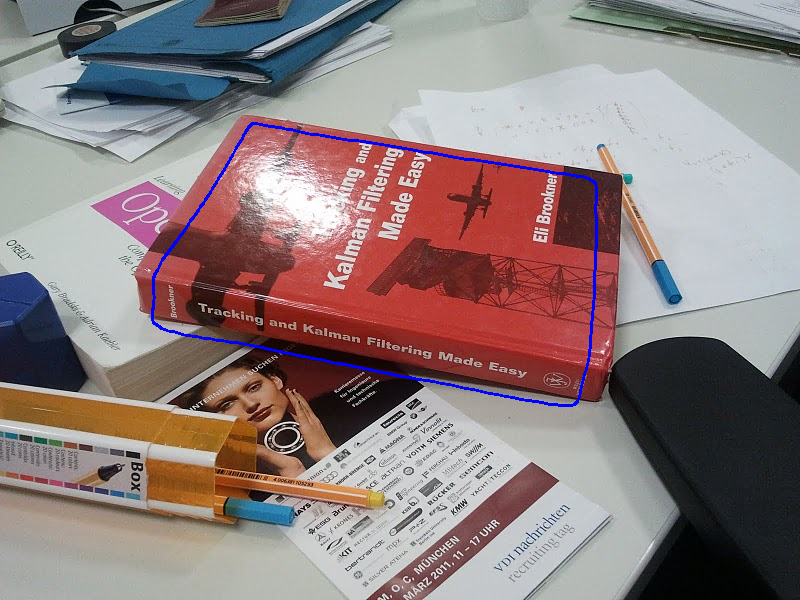
\includegraphics[width=2.0in]{images/book/0.png}}    
  \end{minipage}% 
  \begin{minipage}[t]{0.45\linewidth} 
    \centering 
    \subfloat[iteration 2]{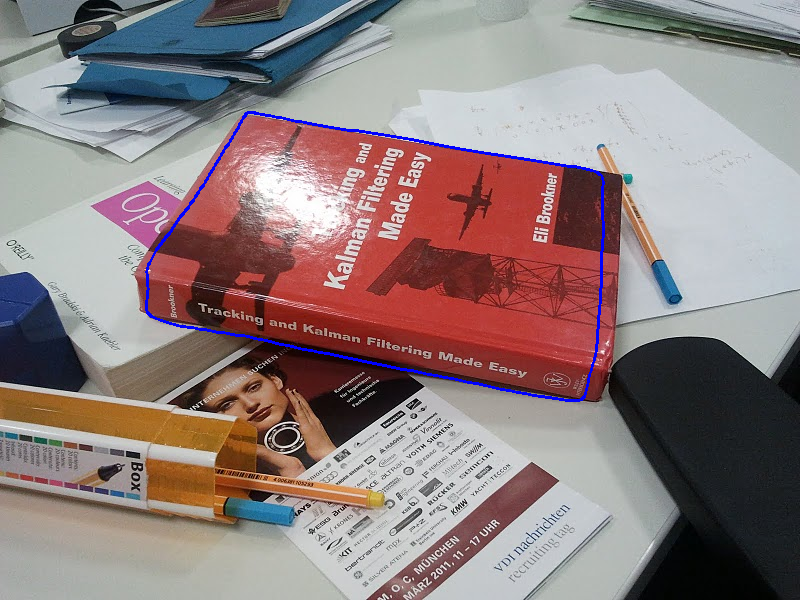
\includegraphics[width=2.0in]{images/book/1.png}}
  \end{minipage} 
  \begin{minipage}[t]{0.45\linewidth} 
    \centering 
    \subfloat[iteration 3]{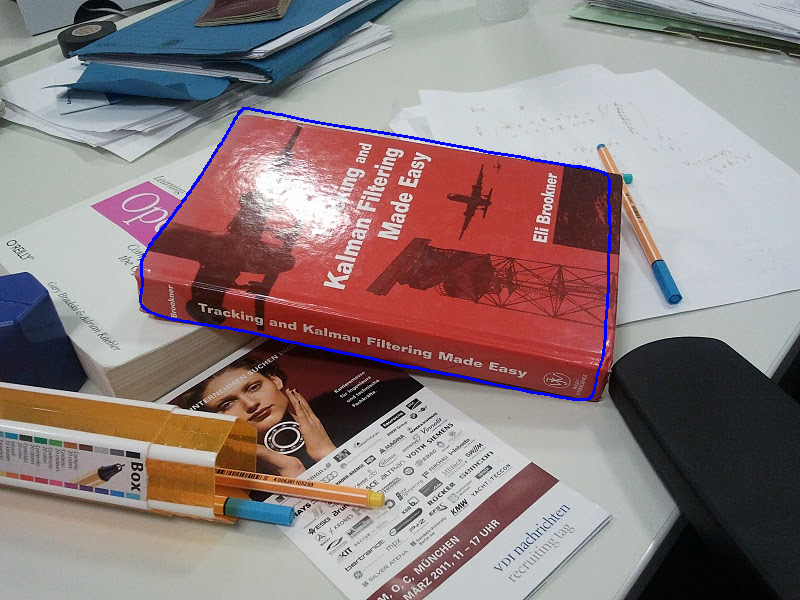
\includegraphics[width=2.0in]{images/book/2.png}}
    \label{subfig:iteration 3}
  \end{minipage} 
  \begin{minipage}[t]{0.45\linewidth} 
    \centering 
    \subfloat[iteration 14]{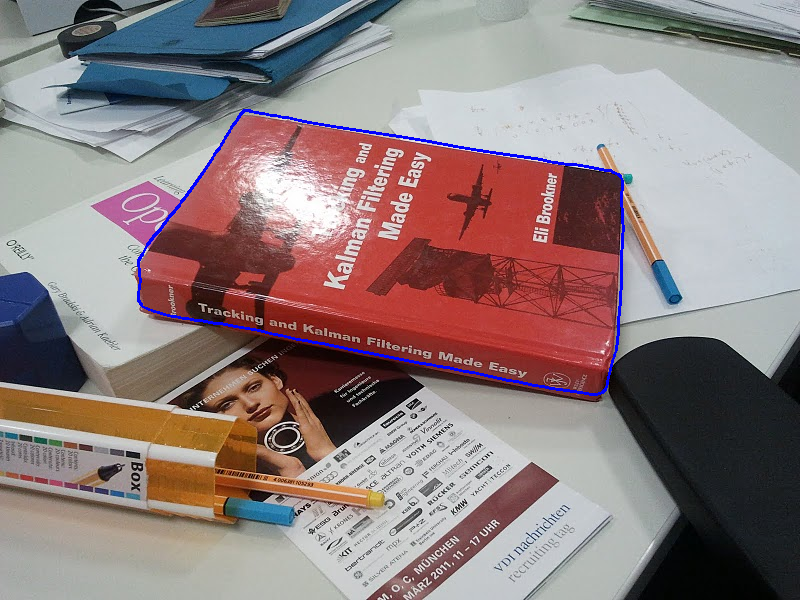
\includegraphics[width=2.0in]{images/book/13.png}}
  \end{minipage} 
\caption{Fitting a rigid wire frame}
\end{figure}


\section{Tracking initialization from sift features}

Scale-invariant feature transform (or SIFT) is an algorithm to detect
and describe local features in images.  It is widely used to solve
many problems in the field of computer vision, such as object
recognition, robotic mapping and navigation, video tracking, and match
moving. There are four key stages in the sift algorithm\cite{lowe2004distinctive}:
\begin{enumerate}
\item \textbf{Scale-invariant feature detection}: an image is transformed into
  a collection of vectors which are scale-invariant. By applying a difference-of-Gaussian
function to a series of smoothed and resampled images, potential
interest can be identified.
\item \textbf{Keypoint localization and indexing}: keypoints are selected at given
  candidate location, then store SIFT keys and identifying matching keys from the new image
\item \textbf{Orientation assignment}:  based on local image gradient
  directions each keypoint is assigned one or more orientations.
\item \textbf{Keypoint descriptor}: measure the local image gradients
  at the selected scale in the region around each keypoint
\end{enumerate}


The SIFT keypoints and features are local and based on the appearance
of the object at particular interest points. The SIFT algorithm has following
features and advantages:
\begin{itemize}
\item invariant to image scale and rotation, robust to changes in
  illumination and minor changes in viewpoint
\item highly distinctive, easy to extract,allow for correct object
  identification and easy to match against a database of local
  features. 
\item need few features (as few as 3) from an object to compute its location
  and pose. Computation cost is moderate on modern computer hardware.
\end{itemize}

Based on these features, SIFT is usable for object recognition, the
steps are given below.
\begin{itemize}
\item extract SIFT features from a series of input template image,
  then store these features into a database.
\item given a new input image, by using the algorithm, the features in
  the image are matched to the SIFT feature database obtained from the
  training images.
\end{itemize}

In this thesis, we plan to use the SIFT algorithm to initialize the
contour of an object. Assume we have marked the boundary points in the
training images. In order project these boundary points to a image
being studied, it is essential to estimate the homography between the
images. The SIFT is helpful for realize this. However, SIFT matching
in the step 2 above might leads to lots of "false" matches. In order
to evaluate the homography, firstly we have to exclude the
mismatches. 

RANSAC is a good approach for this and ideal partner of SIFT. It is a
iterative process by randomly select enough matches to fit
homography. It contains following stages \cite{fischler1981random}.
\begin{itemize}
\item  Randomly select a sample of matched points and instantiate the
  model from this subset
\item Determine the set of data points that are within a distance
  threshold of the homography. The set is the consensus set of the sample
  and defines the inliers.
\item If the size of the set (e.g. the number of inliers) is greater
  than some threshold, re-estimate the homography using all the matched
  points and terminate. Otherwise, select a new subset and repeat the
  above.
\item After some trials the largest consensus set is selected, and the
  homography is re-estimated using all the points in the subset.
\end{itemize}

One fast way to compute the homography in a least squares sense is to use the Normalized
Direct Linear Transform (normalized
DLT)\cite{hartley2003multiple}. The Normalized DLT algorithm computes
a homography for a projective transformation by using at least 4 point
correspondences and then minimizing corresponding norm.

After obtaining the homography between the template image and the
image being studied, the contour of object can be easily projected
into the target image to obtain the estimate of the contour
position. This is illustrated in Figure \ref{fig:sift} on page
\pageref{fig:sift} and \ref{fig:sift_result} on page
\pageref{fig:sift_result}. Note that because SIFT is only invariant for
minor changes in view points, the method does not always work for
non-planar object which have different viewpoint from the one in the
template image. Hence, those objects in our examples are planar.

\begin{figure}[htbp]
  \centering
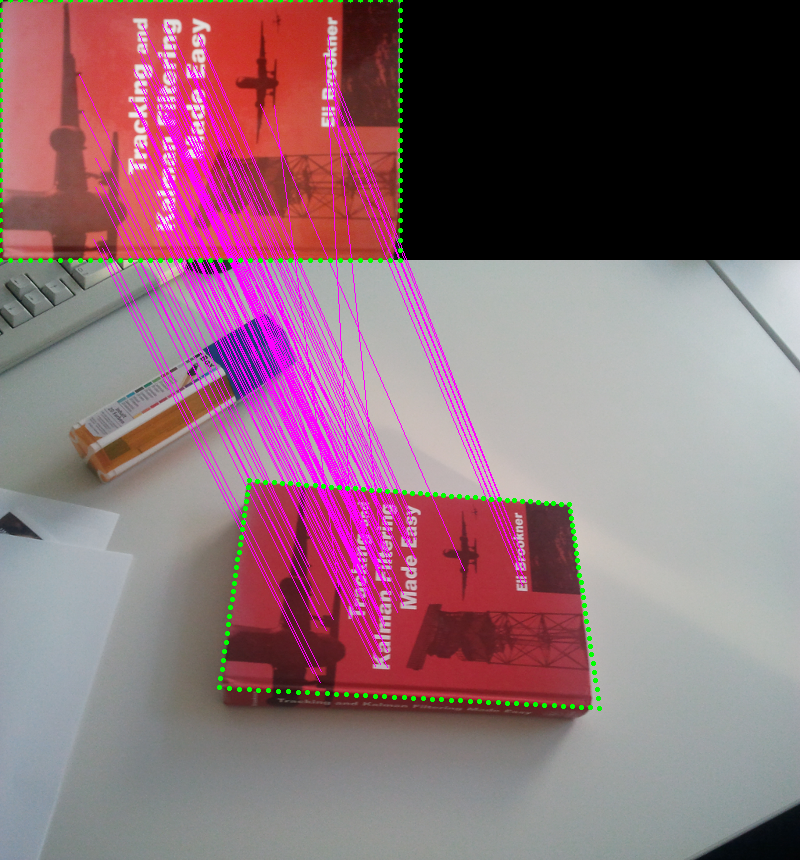
\includegraphics[width=\linewidth]{images/sift.png}
\caption{sift contour initialization}
\label{fig:sift}
\end{figure}

\begin{figure}[htbp]
  \centering
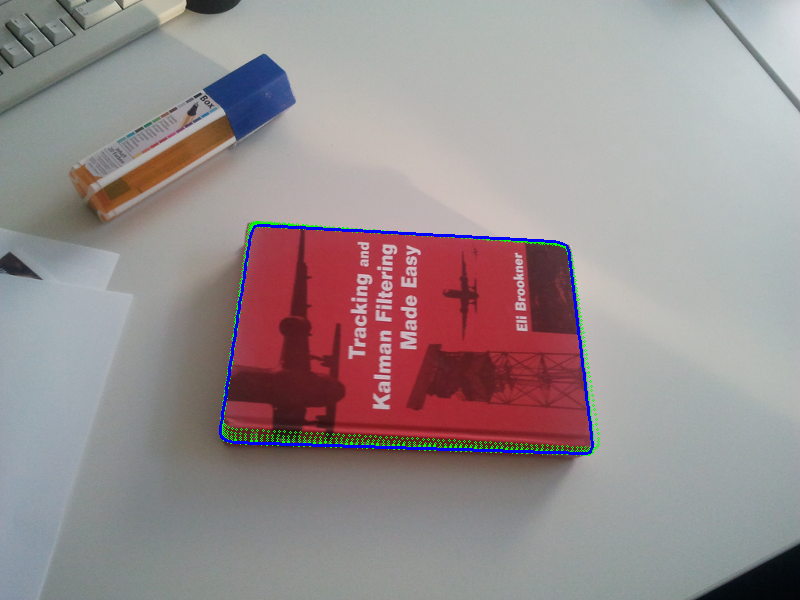
\includegraphics[width=\linewidth]{images/sift_result.png}
\caption{sift contour initialization}
\label{fig:sift_result}
\end{figure}


\section{Tracking initialization from 3D point cloud}
\label{sec:tifpc}
A point cloud is a set of vertices in a three-dimensional coordinate system. These vertices are usually defined by X, Y, and Z coordinates, and typically are intended to be representative of the external surface of an object.
Point clouds are most often created by 3D scanners. These devices measure in an automatic way a large number of points on the surface of an object, and often output a point cloud as a data file. The point cloud represents the set of points that the device has measured.
As the result of a 3D scanning process point clouds are used for many purposes, including to create 3D CAD models for manufactured parts, metrology/quality inspection, and a multitude of visualization, animation, rendering and mass customization applications.
While point clouds can be directly rendered and inspected,[1] usually point clouds themselves are generally not directly usable in most 3D applications, and therefore are usually converted to polygon or triangle mesh models, NURBS surface models, or CAD models through a process commonly referred to as surface reconstruction. There are many techniques for converting a point cloud to a 3D surface. Some approaches, like Delaunay triangulation, alpha shapes and ball pivoting, build a network of triangles over the existing vertices of the point cloud, while other approaches convert the point cloud into a volumetric distance field and reconstruct the implicit surface so defined through a marching cubes algorithm.[2]
One application in which point clouds are directly usable is industrial metrology or inspection. The point cloud of a manufactured part can be aligned to a CAD model (or even another point cloud), and compared to check for differences. These differences can be displayed as color maps that give a visual indicator of the deviation between the manufactured part and the CAD model. Geometric dimensions and tolerances can also be extracted directly from the point cloud.
Point clouds can also be used to represent volumetric data used for example in medical imaging. Using point clouds multi-sampling and data compression is achieved.[3]
In geographic information system, point clouds are one of the sources
to make digital elevation model of the terrain.[4] The point clouds
are also employed in order to generate 3D model of urban environment,
e.g.[5]

employed in order to generate 3D model of urban environment e.g.



